\documentclass[tikz,border=10pt]{standalone}
\usepackage{tkz-euclide} % 增强几何绘图功能
\begin{document}
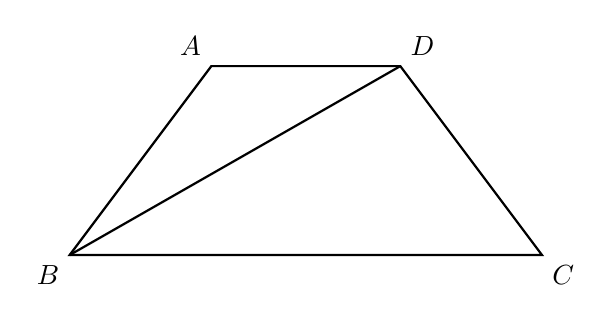
\begin{tikzpicture}[scale=1.2, thick, >=stealth]    
% 1. 定义顶点坐标 (根据视觉比例设定)    
% 设定 B 为原点，底边 BC 长度为 5，高为 2    
\coordinate (B) at (0, 0);    
\coordinate (C) at (5, 0);    
\coordinate (A) at (1.5, 2);    
\coordinate (D) at (3.5, 2);
    % 2. 绘制梯形外框 ABCD    
\draw (A) -- (B) -- (C) -- (D) -- cycle;
    % 3. 绘制对角线 BD    
\draw (B) -- (D);
    % 4. 标注顶点标签    
% 使用 anchor 自动调整文字位置，避免覆盖图形    
\node[above left]  at (A) {$A$};    
\node[below left]  at (B) {$B$};    
\node[below right] at (C) {$C$};    
\node[above right] at (D) {$D$};
    % 5. (可选) 如果需要强调 AD // BC，可以取消注释下面两行绘制箭头    
% \draw[->] (2.4, 2) -- (2.6, 2);     
% \draw[->] (2.4, 0) -- (2.6, 0);
\end{tikzpicture}
\end{document}